% ============================================================================
%  第 9 章  非阿贝尔（原文 pp.~115--132）
% ============================================================================
\chapter{非阿贝尔}\label{ch:09}

\begin{keytakeaways}
本章要把 Abel 对偶推广到非交换群。直接的障碍是：$G$非交换时群代数$\C G$非交换，于是没有现成的谱分解，也就没有明显的“对偶”对象$\Spec(\C G,*)$；我们必须从别处找到交换性，而它自然来自 TFT。
第一步是把$\mathrm{Pic}(C)$换成非阿贝尔的对应物：主$G$-丛的模空间$\Bun_G(C)$，以及其上的（几何）自守形式。Weil 描述把$\Bun_G$写成整体域上的二重商$G(F)\backslash G(\bA)/G(\cO)$；数域情形给出局部对称空间$\Gamma\backslash G_\R/K$。
由于$\Bun_G$不是群，其函数上没有卷积，对称性改由 Hecke 代数$\cH_{G,K}=\C[K\backslash G/K]$（群胚代数）提供。逐点的局部 Hecke 代数彼此交换，Satake 定理说它是多项式代数；Harish-Chandra 同构给出交换微分算子环作为其无穷小版本。最后以$G=\mathrm{PGL}_2$、$K=\Q_p$的 Bruhat--Tits 树为例，把这一切画成树上的“径向平均”算子。
\end{keytakeaways}

\begin{flushright}\small 第 17 讲；2021 年 3 月 30 日\end{flushright}

我们的目标是为非交换群发展 Abel 对偶的类比。基本问题是：若从非交换的$G$出发，则群代数$\C G$非交换，于是并不立刻有谱分解的理论，也就没有明显的“对偶”概念——因为以前对偶就是$\Spec(\C G,*)$。所以我们需要在某处找到某种交换性，以便描述某种对偶。这种交换性会以自然的方式从 TFT 来到我们这里。

可以从场论出发，但我们改从最终要解决的“问题”出发。基本上，第一个问题是我们需要把$\mathrm{Pic}(C)$换成某个非阿贝尔的对应物，这就是自守形式的理论。

% ================================================================
\section{自守形式}\label{sec:9.1}
\begin{sectionkey}
把线丛换成主$G$-丛，就得到非阿贝尔几何类域论的舞台$\Bun_G(C)$。在有限域上取函数得到（非分歧）自守函数，取上同调得到上同调自守形式；在一般域上取层则得到几何自守形式。Weil 定理把$\Bun_G$实现为二重商，从而暴露出大量 Hecke 对称性。
\end{sectionkey}

\subsection{$G$-丛}
\begin{sectionkey}
主$G$-丛是局部平凡、带$G$-作用的纤维丛；其模空间$\Bun_G(C)$在$G=\GG_m$时还原 Picard 栈。
\end{sectionkey}

设$C$是域$k$上的光滑射影曲线。我们主要关心有限域情形$k=\F_q$，或$k=\C$——此时研究的是紧 Riemann 面。在几何 CFT 中，我们研究$\mathrm{Pic}(C)$上的函数（$k=\F_q$情形）或层（一般情形），而$\mathrm{Pic}(C)$由$C$上线丛的同构类组成。

把线丛换成向量丛，或更一般地换成所谓\term{主 $G$-丛}{principal $G$-bundle}，就得到非阿贝尔类比。设$G$是$k$上的代数群。我们通常要求它仿射，但之后甚至会假设它约化。\footnote{目前只需把“约化”理解为：$G$是熟悉的 Lie 群之一，如$\mathrm{GL}_n,\mathrm{SO}_n,\mathrm{Sp}_n,\dots$}则$C$上的主$G$-丛是丛
\begin{equation}\tag{9.1}
\begin{array}{c}
P\\
\downarrow\\
C
\end{array}
\end{equation}
带$G$-作用，并使得局部地\footnote{一般地这其实应是 \'etale 局部，但在曲线上用 Zariski 拓扑就足够了。}在开集$U$上丛看起来是平凡的：
\begin{equation}\tag{9.2}
P|_{U}\simeq U\times G.
\end{equation}

\begin{srcex}{41}
若$G=\mathrm{GL}_n$，则$C$上的主$G$-丛就是$C$上秩$n$的向量丛。
\end{srcex}

现在可以考虑模空间$\Bun_G(C)$，它其实是$C$上主$G$-丛的模空间（或栈）。其$R$-点由
\begin{equation}\tag{9.3}
\Bun_G(C)(R)=\{C\times\Spec R\ \text{上的 }G\text{-丛}\}/\sim
\end{equation}
给出，即$C$上$G$-丛的$R$-族。

\begin{srcex}{42}
$G=\mathrm{GL}_1=\GG_m$的情形还原 Picard 栈：
\begin{align}
\Bun_{\mathrm{GL}_1}(C)&=\mathrm{Pic}(C)\tag{9.4}\\
&=|\mathrm{Pic}(C)|\times pt/\GG_m.\tag{9.5}
\end{align}
\end{srcex}

所以对曲线$C$我们附着这个空间$\Bun_G(C)$，然后在这个空间上做函数论，这就是非阿贝尔几何 CFT。

\subsection{自守函数}
\begin{sectionkey}
在有限域上忘掉栈结构，得到$G$-丛同构类的离散集；其上的（带增长条件的）函数即非分歧自守函数。
\end{sectionkey}

设$k=\F_q$是有限域，考虑$\Bun_G(C)(\F_q)$。我们可以忘掉栈结构，得到$G$-丛同构类的离散集$|\Bun_G(C)(\F_q)|$。

\begin{srcdef}{2}
$C$上关于$G$的（非分歧）\term{自守函数}{automorphic function}是
\begin{equation}\tag{9.6}
|\Bun_G(C)(\F_q)|
\end{equation}
上的函数，可能带增长条件，例如紧支撑。
\end{srcdef}
% [Tutor Note: 原文此处误写作$\Bun_g(C)(\F_q)$（下标小写$g$），应为$\Bun_G$。另注意“非分歧”指只允许在$C$的有限多个点上分歧；一般情形还需要在指定分歧除子处引入 level 结构，参见 9.1.3 节末的 level $N$ 版本。]

\subsection{Weil 描述}
\begin{sectionkey}
$G$-丛在一般点处平凡、在任意点处形式平凡，两组平凡化在重叠处给出限制直积中的元素，于是$\Bun_G$被实现为二重商$G(F_C)\backslash\prod'_xG(K_x)/\prod G(\cO_x)$。数域情形完全类似，只需把$K_x$换成$\Q_p$或$\R$。
\end{sectionkey}

这个描述对任何域都成立。首先要说的是：$C$上的$G$-丛在一般点处平凡，即任何$P\to C$都有有理截面，也就是说它可以在某个有限点集之外被平凡化。另一说法是：任何$G$-丛在任意$x\in C$附近都是形式平凡的，即它可以在任意点附近被平凡化。由所有这些数据，我们得到
\begin{equation}\tag{9.7}
\prod_{x\in C}{}^{\prime}\,G(K_x)
\end{equation}
中的一个元素，具体如下。对$x\in C$有 Taylor 级数的完备局部环$\cO_x$，它位于 Laurent 级数的局部域中：$\cO_x\subset K_x$。于是我们有一个丛、一个在某个点之外处的平凡化、一个在该点附近的平凡化；在重叠处，两个平凡化之差定义了$G(K_x)$中的一个元素。限制直积
\[
\prod{}^{\prime}
\]
的意思是：除有限多个$x$之外，我们得到的是$G(\cO_x)$而非$G(K_x)$中的元素。

定理如下。

\begin{srcthm}{5}（Weil）
对$k=\F_q$，
\begin{align}
|\Bun_G(C)(k)|&=G(F_C)\backslash\prod_{x\in C}{}^{\prime}G(K_x)\Big/\prod G(\cO_x)\tag{9.8}\\
&=G(F_C)\backslash G(\bA_C)/G(\cO_{\bA_C}).\tag{9.9}
\end{align}
\end{srcthm}

% ---------------------------------------------------------------- 原文 p.117
回忆这与 5.2.2 节中的陈述相同。\term{Beauville--Laszlo 定理}{Beauville--Laszlo theorem}说，我们确实可以用形式过渡数据粘出一个$G$-丛：若有一个点周围圆盘上的丛、该点之外的丛、以及它们之间的过渡数据，就得到整体上真正的丛。这并非自动成立，因为这不是一个真正的开覆盖（形式幂级数的$\Spec$并不是开集）。

回忆 Abel 情形，对点$x\in C$我们有局部因子
\begin{equation}\tag{9.10}
|\mathrm{GL}_1(K_x)/\mathrm{GL}_1(\cO_x)|=\bigl|K_x^{\times}/\cO_x^{\times}\bigr|\simeq\Z,
\end{equation}
即这些商仍是群。这是线丛除子描述的来源。非阿贝尔情形我们改为所谓\term{仿射 Grassmann 流形}{affine Grassmannian}
\begin{equation}\tag{9.11}
\Gr_G=G(K_x)/G(\cO_x).
\end{equation}
这不是群，因为我们不再模去正规子群。可以把它想成由$C$上的一个$G$-丛以及$C\setminus x$上的一个平凡化组成。

这个 Weil 定理在数域设定中有显然的类比。

\subsection*{数域版本}
首先要确定的是理元类群的$G$-类比。设$F/\Q$是有限扩张，例如$F=\Q$。则我们要写一个与前面类似的二重商：
\begin{equation}\tag{9.12}
G(\Q)\backslash G(\bA_\Q)/G(\cO_{\bA_\Q}).
\end{equation}
回忆域$F$的\term{阿黛尔环}{adèle ring}是
\begin{equation}\tag{9.13}
\bA_F=\prod_{v}{}^{\prime}F_v.
\end{equation}
对$\Q$的情形：
\begin{equation}\tag{9.14}
\bA_\Q=\prod_{p}{}^{\prime}\Q_p\times\R,
\end{equation}
其中
\begin{equation}\tag{9.15}
\prod_{p}{}^{\prime}\Q_p=\bA_{\mathrm{fin}}=\widehat{\Z}\otimes_{\Z}\Q
\end{equation}
是有限阿黛尔。因此有
\begin{equation}\tag{9.16}
G(\bA_\Q)=G(\bA_{\mathrm{fin}})\times G(\R).
\end{equation}
注意
\begin{equation}\tag{9.17}
G(\Q)\subset G(\bA_\Q)
\end{equation}
构成离散子群。于是可以构造
\begin{equation}\tag{9.18}
G(\Q)\backslash G(\bA_\Q)/G(\widehat{\Z})\times K_\infty,
\end{equation}
其中$K_\infty\subset G(\R)$紧。可以把这看成$\Bun_G(\Q)$所扮演的角色。这里有一个自然的子群要考虑。首先注意实 Lie 群是子群$G(\R)\hookrightarrow G(\bA_\Q)$。在左边我们要模去
\begin{equation}\tag{9.19}
\prod{}^{\prime}G(\Q_p)\supset G(\Q)\cap\prod G(\Z_p)=G(\Z).
\end{equation}

% ---------------------------------------------------------------- 原文 p.118
于是由初等代数得到
\begin{equation}\tag{9.20}
G(\Z)\backslash G(\R)/K_\infty\hookrightarrow G(\Q)\backslash G(\bA_\Q)/G(\widehat{\Z})\times K_\infty.
\end{equation}
断言是：这是一个连通分支，并且对一类合宜的群（单连通、半单），这将是双射。\footnote{原文此处右侧有橙色批注：“cite: M. Emerton: classical and $p$-adic modular forms.”（提示引用 M. Emerton 的《经典与 $p$-进模形式》。）}

这里最基本的情形是$G=\mathrm{GL}_2$。于是我们要问的是类似$\Bun_2(\Spec\Z)$的东西，这只是“在$\infty$处平凡化的秩$2$$\Z$-模”的诗意记号。
设$\mathcal B$由$\R^{2}=\C$的$R$-基组成，即
\begin{align}
\mathcal B&\simeq\mathrm{Iso}_{\R}\bigl(\Z^{2}\otimes_{\Z}\R,\R^{2}\bigr)=\mathrm{GL}_2\R\tag{9.21}\\
&\simeq\C^{\times}\times\C\setminus\R.\tag{9.22}
\end{align}
与最后一行的同构由基$(z_1,z_2)$送到对$(z_1,z_2/z_1)$给出。

现在可以考虑（更有趣的）空间
\begin{equation}\tag{9.23}
\mathcal L=\C\simeq\R^{2}\ \text{中的格}.
\end{equation}
这样的格是自由秩$2$的$\Z$-模，并带同构$\Lambda\otimes_{\Z}\R\xrightarrow{\sim}\C$。这等同于
\begin{equation}\tag{9.24}
\mathcal L=\mathrm{GL}_2\Z\backslash\mathcal B,
\end{equation}
即我们模去$\mathrm{GL}_2\Z$在$\Lambda\simeq\Z^{2}$上的作用。应把$\mathcal L$看成$\Spec\Z$上秩$2$丛（在无穷远处平凡化）的一个版本。

$\mathcal L$有各种变体，例如$\mathcal L(N)$由格连同模$N$的一个固定基组成：
\begin{equation}\tag{9.25}
\mathcal L/N\simeq(\Z/N\Z)^{\oplus 2},
\end{equation}
即秩$2$丛连同$(N)\subset\Spec\Z$上的一个平凡化。还有$\overline{\mathcal L}$，由格模去$\C$-位似组成，于是
\begin{equation}\tag{9.26}
\overline{\mathcal L}=\mathrm{GL}_2\Z\backslash\mathcal B/\C^{\times}=\mathrm{PSL}_2\Z\backslash\mathbb H.
\end{equation}

\begin{srclem}{6}
$\mathcal L\simeq\mathrm{GL}_2\Q\backslash\mathrm{GL}_2\bA/\mathrm{GL}_2\cO_\bA$。
\end{srclem}
这个引理依赖两件事：
\begin{itemize}
\item $\mathrm{GL}_2\Z=\mathrm{GL}_2\Q\cap\mathrm{GL}_2\widehat{\Z}$，以及
\item $\mathrm{GL}_2(\bA_{\mathrm{fin}})=\mathrm{GL}_2(\cO_\bA)\mathrm{GL}_2\Q$。
\end{itemize}
其想法是：从$\mathcal L\simeq\mathrm{GL}_2\Z\backslash\mathrm{GL}_2\R$出发，然后要在右边再模去另一个子群。一个选择是极大紧子群$\mathrm{O}_2\subset\mathrm{GL}_2\R$；也可以取中心$\R^{\times}\subset\mathrm{GL}_2\R$。二者合起来“撑开”我们以前模去的这个$\C^{\times}$。经典模形式就出现在这里：它们是$\mathrm{PSL}_2(\Z)\backslash\mathbb H$上某个线丛的全纯截面，外加增长条件。它们坐在$\mathrm{GL}_2(\Z)\backslash\mathcal L$上所有函数构成的空间里：
\begin{equation}\tag{9.27}
\mathrm{GL}_2(\Z)\backslash\mathcal L.
\end{equation}
$\mathrm{GL}_2/\Q$的\term{自守形式}{automorphic form}是
\begin{equation}\tag{9.28}
\mathrm{GL}_2\Q\backslash\mathrm{GL}_2\bA/\mathrm{GL}_2\cO_\bA
\end{equation}
上的函数$\varphi$，

% ---------------------------------------------------------------- 原文 p.119
它在$\mathrm{GL}_2\R$上光滑，并满足增长条件。这个增长条件是无穷素位$\R$上的条件。我们也可以做 level $N$ 的版本，此时改为取
\begin{equation}\tag{9.29}
\mathrm{GL}_2\Q\backslash\mathrm{GL}_2\bA/\mathrm{GL}_2\cO_\bA^{(N)}
\end{equation}
上的函数。

\begin{srcex}{43}
这对其他群也成立。考虑正交丛的模空间。固定一个偶格，即自由$\Z$-模$V$与二次型
\begin{equation}\tag{9.30}
q\colon V\to\Z.
\end{equation}
于是可以定义正交群：
\begin{equation}\tag{9.31}
\Aut(V,q)=\mathrm{O}_q(\Q)\backslash\mathrm{O}_q(\bA)/\mathrm{O}_q(\cO_\bA).
\end{equation}
它由$q$的亏格中的二次型的同构类组成。这意味着我们考虑的是“模每个$N$都与$q$等同”的二次型。
\end{srcex}

所以对任何$G$与$F$，可以写出$F$上的$\Bun_G$：
\begin{equation}\tag{9.32}
G(F)\backslash G(\bA_F)/G(\cO_\bA)\times K_\infty.
\end{equation}
在有限域上的函数域设定中，这是离散集，所以不必担心在这个空间上取什么样的函数。现在它看起来像“实 Lie 群模去极大紧子群与一个格”。具体如下。$F$的 Archimedes 完备化是
\begin{equation}\tag{9.33}
F\otimes_{\Q}\R=\R^{\times s_1}\times\C^{\times s_2}.
\end{equation}
于是$G$的 Archimedes 部分是如下实 Lie 群，记作$G_\R$：
\begin{equation}\tag{9.34}
G_\R=G(F\otimes_{\Q}\R)=G(\R)^{\times s_1}\times G(\C)^{\times s_2}.
\end{equation}
所以我们要看的是空间
\begin{equation}\tag{9.35}
[G]_F:=\Gamma\backslash G_\R/K,
\end{equation}
其中$K$极大紧，$\Gamma=G(\cO_F)$是格。这称为\term{算术局部对称空间}{arithmetic locally symmetric space}。为避免指定函数类型，我们可以直接过渡到上同调。
% [Tutor Note: (9.33)–(9.34) 中上标“$\times s_i$”是原文记号，读作“取$s_i$个拷贝”（即$(\R^\times)^{s_1}\times(\C^\times)^{s_2}$等）。这里$s_1$是$F$的实素位个数，$s_2$是复素位个数，故$[F:\Q]=s_1+2s_2$。]

\subsection{上同调自守形式}
\begin{sectionkey}
把函数换成上同调，就不必操心函数类型。对紧致的局部对称空间，$H^*([G]_F)$就是群上同调$H^*(G(\Z),\C)$；Eichler--Shimura 同构说明经典模形式坐在$\mathrm{SL}_2$的上同调自守形式中。
\end{sectionkey}

现在我们从函数过渡到上同调，这样就不必关心所考虑函数的类型。这导致\term{上同调自守形式}{cohomological automorphic forms}：
\begin{equation}\tag{9.36}
H^{*}\bigl(G(F)\backslash G(\bA)/G(\cO)\times K\bigr).
\end{equation}
在小心处理连通分支之后，这是
\begin{equation}\tag{9.37}
H^{*}\bigl(G(F)\backslash G(\bA)/G(\cO)\times K\bigr)=H^{*}\bigl([G]_F=G(\Z)\backslash G_\R/K\bigr).
\end{equation}
这个局部对称空间可缩，所以
\begin{equation}\tag{9.38}
H^{*}([G]_F)=H^{*}(G(\Z),\C)
\end{equation}
% [Tutor Note: (9.37)–(9.38) 中的$G(\Z)$应理解为$\Gamma=G(\cO_F)$：对一般数域$F$，整环是$\cO_F$，$G(\Z)$只是$F=\Q$时的写法。作者在此沿用$\Q$的记号。]
只是群上同调。更一般地，对$G(\Z)$作用在$V_\C$上，可以把上式换成
\begin{equation}\tag{9.39}
H^{*}(G(\Z),V_\C)=H^{*}\bigl([G]_F,\text{局部系统}\bigr).
\end{equation}

有一个所谓 \term{Eichler--Shimura 同构}{Eichler--Shimura isomorphism}（即$\mathrm{SL}_2\Z\backslash\mathbb H$上的 Hodge 理论），它说经典模形式坐在$\mathrm{SL}_2$的上同调自守形式中。所以不必谈论带增长条件的全纯函数，我们可以把一切实现在上同调中。

回忆函数域情形中$[G]_F$的类比是$\Bun_G(C)(\F_q)$，然后我们取函数。但离散集的上同调就是其上的函数：
\begin{equation}\tag{9.40}
\mathrm{Funct}\bigl(\Bun_G(C)(\F_q)\bigr)=H^{*}\bigl(\Bun_G(C)(\F_q)\bigr).
\end{equation}

\subsection{几何自守形式}
\begin{sectionkey}
用层替换函数就得到几何自守形式$\Shv(\Bun_G(C))$，即自守层；它应当在 TFT 中出现在曲面层面，正如 Abel 情形中的$\Sigma\mapsto\Shv(\mathrm{Pic}\,\Sigma)$。由于$\Bun_G$不是群，Hecke 算子不交换，因此不能直接做谱分解——这正是需要 TFT 的地方。
\end{sectionkey}

更一般地，我们可以考虑“几何”自守形式。这与几何 CFT 含义相同：我们研究层而非函数。于是对任何域$k$与$C/k$，\term{几何自守形式}{geometric automorphic forms}是
\begin{equation}\tag{9.41}
\Shv(\Bun_G(C)).
\end{equation}
这些就是所谓的自守层。我们希望它出现在曲面层面的 TFT 中，因为它类似于 Abel 故事中的
\begin{equation}\tag{9.42}
\Sigma\mapsto\Shv(\mathrm{Pic}\,\Sigma).
\end{equation}

\begin{srcrem}{45}
这个自守层范畴将成为我们的基本研究对象之一。一个动机来源是：它直接推广了我们以前的东西——把$\mathrm{GL}_1$换成$\mathrm{GL}_n$就得到这些丛的模空间，我们可以试着对它们做在 CFT 中做过的事。另一个动机来源是数域情形：那里的丛空间正是我们从数论中看到的局部对称空间。
\end{srcrem}

基本问题在于：与$\mathrm{Pic}=\Bun_{\mathrm{GL}_1}$不同，$\Bun_G$不是群，甚至没有自然作用其上的群：当我们构造
\begin{equation}\tag{9.43}
\mathrm{SL}_2\Z\backslash\mathbb H=\mathrm{SL}_2\Z\backslash\mathrm{SL}_2\R/\mathrm{SO}_2
\end{equation}
时，两侧都模去了群，所以没有余地让别的东西作用。我们会发现存在称为 Hecke 算子的东西确实在作用，但它们不交换，所以不能完全做谱分解。这就是我们将用到 TFT 想法之处。

\begin{flushright}\small 第 18 讲；2021 年 4 月 1 日\end{flushright}
% [Tutor Note: 原文此处在“This is where we will use ideas from TFT.”之后标有橙色批注“transition”，提示讲次过渡；本译本以讲次标记保留该信息。]

回忆我们有这个阿黛尔一致化图景：
\begin{align}
|\Bun_G(C)(\F_q)|&=G(F_C)\backslash\prod_{x}{}^{\prime}G(K_x)\Big/\prod G(\cO_x)\tag{9.44}\\
&=G(F_C)\backslash G(\bA_C)/G(\cO_\bA).\tag{9.45}
\end{align}
然后我们要研究其上的函数。这是离散集，所以所取函数的概念没有歧义。但我们想在某些作用下分解它们，所以需要回答下面的问题。

\medskip
\noindent\textbf{问题 2.}\ 什么作用在自守形式上？

% ---------------------------------------------------------------- 原文 p.121
问题在于$\Bun_G$不是群；而当$G=\mathrm{GL}_1$时$\Bun_G=\mathrm{Pic}$自然是群，所以其上的函数有卷积的概念。幸运的是，这个空间具有形式$X/K$，其中$X$是带群$G$作用的空间，$K\subset G$是子群。所以我们从带$G$-对称性的空间$X$出发，现在的问题是：$X/K$上剩下什么对称性？在我们的情形，出发点是限制直积$\prod'_{x\in C}G(K_x)$，在右边模去 Taylor 级数群$G(\cO_x)$，再在左边模去整体域$G(F_C)$。所以我们有巨量的对称性：在曲线上每一点都有$G(K_x)$，而我们只模去了它“一半”，即每点的 Taylor 级数。我们也可以改为构造理元类群的类比
\begin{equation}\tag{9.46}
G(F_c)\backslash\prod{}^{\prime}G(K_x),
\end{equation}
其中右边不模去，于是有巨群
\begin{equation}\tag{9.47}
\prod G(K_x)
\end{equation}
的作用，而且它们彼此全部交换。也就是说，$G(K_x)$本身非交换，但各个副本之间交换。所以我们有巨量对称性。当我们再模去 Taylor 级数部分$\prod G(\cO_x)$时，可以希望其中一部分对称性保留下来。这正是 Hecke 代数的想法：它们捕捉这种残余对称性。

% ================================================================
\section{Hecke 代数}\label{sec:9.2}
\begin{sectionkey}
对有限群$G$作用在有限集$X$上、$K\subset G$，$X/K$上的函数即$K$-不变量$\C[X]^K$；其自同构（作为函子）由$\C[K\backslash G/K]$表示，这就是 Hecke 代数。它在球表示子范畴上与$\Rep(G)$等价，并在一般设定中给出双陪集代数、群胚代数与卷积结构。
\end{sectionkey}

设$G$是作用在有限集$X$上的有限群，$K\subset G$是子群。这些假设只是为了方便；我们将看到的特征会推广到其他设定。我们要回答的问题是：

\medskip
\noindent\textbf{问题 3.}\ 什么作用在$\C[X/K]$上？

你在群论中最先学到的答案是$K$在$G$中的正规化子$N_G(K)$。但有时$N_G(K)=K$，它平凡地作用。所以这真的只有在按群的元素来思考时才是正确答案。相反，我们应该按群代数$\C G$来思考。$\C G$作用在$X$上的函数上，而$X/K$上的函数等同于$X$上的$K$-不变函数：
\begin{equation}\tag{9.48}
\C[X/K]=\C[X]^{K}.
\end{equation}
现在我们要理解$G$-表示的$K$-不变量，即把
\begin{equation}\tag{9.49}
(-)^{K}\colon\Rep G\to\Vect
\end{equation}
看成函子，并想理解它的自同构$\End\bigl((-)^{K}\bigr)$。每当你想要计算函子的自同构时，都应当问它是否可表示（好的函子可表示），即是否存在$G$-表示$V_{G,K}$使得
\begin{equation}\tag{9.50}
(-)^{K}=\Hom(V_{G,K},-).
\end{equation}
要点是 $\Hom$-$\otimes$伴随给出
\begin{equation}\tag{9.51}
V^{K}=\Hom_{\C K}(\C,V|_{K})=\Hom_{\C G}(\C G\otimes_{\C K}\C,V).
\end{equation}
% [Tutor Note: (9.51) 原文印作“$\C G\otimes_{\C K}\otimes\,\C$”，多了一个$\otimes$，应为$\C G\otimes_{\C K}\C$；此处已按数学含义排版，特此说明。]

% ---------------------------------------------------------------- 原文 p.122
这是 Frobenius 互反律的一个版本：
\begin{equation}\tag{9.52}
\Hom_{\C K}\bigl(\C,\operatorname{Res}^{K}_{G}V\bigr)=\Hom_{\C G}\bigl(\operatorname{Ind}^{G}_{K}\C,V\bigr).
\end{equation}
结论是，表示$(-)^K$的对象是
\begin{equation}\tag{9.53}
V_{G,K}=\operatorname{Ind}^{G}_{K}\C=\C G\otimes_{\C K}\C.
\end{equation}
可以把它想成
\begin{align}
V_{G,K}&=\operatorname{Ind}^{G}_{K}\C=\C G\otimes_{\C K}\C\tag{9.54}\\
&=\{f\colon G\to\C\mid f(gk)=f(g)\}\tag{9.55}\\
&=\C[G/K]=\C[G]^{K},\tag{9.56}
\end{align}
其中我们隐含地用了“有限群上函数与测度相同”这一事实，即我们最终真正得到的应该是$G$上的$K$-不变测度。

\term{Hecke 代数}{Hecke algebra}$\cH_{G,K}$是
\begin{align}
\cH_{G,K}&:=\End\bigl((-)^{K}\bigr)=\End_{\Rep(G)}V_{G,K}=\Hom_{\C G}(V_{G,K},V_{G,K})\tag{9.57}\\
&=(V_{G,K})^{K}=\C[G/K]^{K}\tag{9.58}\\
&=\C[K\backslash G/K].\tag{9.59}
\end{align}
这告诉我们：双陪集上的函数带有典范的代数结构。

有一类特殊的抽象废话（Barr--Beck）说的是下面这件事。我们发现函子$(-)^K$分解为
\begin{equation}\tag{9.60}
\begin{array}{ccc}
\Rep(G) & \xrightarrow{\ (-)^{K}\ } & \Vect\\[2pt]
& \searrow & \nearrow{\scriptstyle\text{Forget}}\\[2pt]
& \cH_{G,K}\text{-mod} &
\end{array}
\end{equation}
可以把$\cH_{G,K}$-mod看成离$\Rep(G)$不太远，即它可能不是等价，但在某类表示上可能是等价。例如我们可以考虑$\Rep(G)$中由$K$-不变量生成的$G$-表示构成的子范畴。比如不可约表示$V$由$K$-不变量生成当且仅当$V^{K}$非平凡。称这些为\term{球表示}{spherical representation}。于是抽象废话告诉我们这是等价：
\begin{equation}\tag{9.61}
\begin{array}{ccc}
\Rep(G) & \xrightarrow{\ (-)^{K}\ } & \cH_{G,K}\text{-mod}\\
\{\text{由 }K\text{-不变量生成}\} & \xleftarrow{\ \sim\ } &
\end{array}
\end{equation}
换一种说法：这个球表示子范畴由$V_{G,K}$生成。也就是说，不可约表示$V$是球的当且仅当它出现在$V_{G,K}$分解为不可约表示的过程中。

% ---------------------------------------------------------------- 原文 p.123
\begin{srcrem}{46}
“球”这个词可追溯到球调和函数的研究。$2$-球面$S^{2}$上的$L^{2}$函数$L^{2}(S^{2})$被$\mathrm{SO}_3$作用。于是可以在该作用下分解$L^{2}(S^{2})$。这有时在高中化学中讲授：不同类型的原子轨道与$\mathrm{SO}_3$的不同不可约表示有关。与我们这里的联系是：$G=\mathrm{SO}_3$，$K=\mathrm{SO}_2$，而$S^{2}=\mathrm{SO}_3/\mathrm{SO}_2$。
\end{srcrem}

现在把$\C[K\backslash G/K]$上的代数结构明确写出。先把群代数$\C G$改写如下。我们有乘法与投影映射：
\begin{equation}\tag{9.62}
\begin{array}{ccc}
& G\times G &\\[-2pt]
\pi_1\swarrow & \downarrow{\scriptstyle\mu} & \searrow\pi_2\\[-2pt]
G & G & G
\end{array}
\end{equation}
于是卷积由下式给出：
\begin{equation}\tag{9.63}
f*h=\mu_{*}\bigl(\pi_1^{*}f\cdot\pi_2^{*}h\bigr).
\end{equation}
我们可以取同一个图并模去$K$，得到
\begin{equation}\tag{9.64}
\begin{array}{ccc}
& K\backslash G\times G/K &\\[-2pt]
\pi_1\swarrow & \downarrow{\scriptstyle\mu} & \searrow\pi_2\\[-2pt]
K\backslash G & K\backslash G/K & G/K
\end{array}
\end{equation}
我们还可以走得更远，对中间的$K$-作用取平衡积。于是得到图
\begin{equation}\tag{9.65}
\begin{array}{ccc}
& K\backslash G\times^{K}G/K &\\[-2pt]
\pi_1\swarrow & \downarrow{\scriptstyle\mu} & \searrow\pi_2\\[-2pt]
K\backslash G/K & K\backslash G/K & K\backslash G/K
\end{array}
\end{equation}
这个图说明我们有双不变函数的子代数
\begin{equation}\tag{9.66}
\C[G]^{K\times K}\subset\C[G].
\end{equation}
群论告诉我们
\begin{equation}\tag{9.67}
K\backslash G/K=G\backslash(G/K\times G/K),
\end{equation}
其中模去对角作用。于是其上的函数是
\begin{align}
\C[K\backslash G/K]&=\C[G/K\times G/K]^{G}\tag{9.68}\\
&\subset\C[G/K\times G/K]\tag{9.69}\\
&=G/K\times G/K\text{-矩阵}.\tag{9.70}
\end{align}

% ---------------------------------------------------------------- 原文 p.124
我们可以如下说明为何称它们为$G/K\times G/K$-矩阵。若$X$是有$n$个元素的有限集，则$\C[X\times X]$就是$n\times n$矩阵，即$\End\C[X]$。于是矩阵乘法有如上所述的推-拉描述：
\begin{equation}\tag{9.71}
\begin{array}{ccc}
& X\times X\times X &\\[-2pt]
\pi_{12}\swarrow & \downarrow{\scriptstyle\pi_{13}} & \searrow\pi_{23}\\[-2pt]
X\times X & X\times X & X\times X
\end{array}
\end{equation}
这一切是说
\begin{equation}\tag{9.72}
(\C G,*)\subset\C[G\times G],\ \text{矩阵},
\end{equation}
而事实上它等于
\begin{equation}\tag{9.73}
\C G=\C[G\times G]^{\mathrm{diag}G}.
\end{equation}

\subsection{群胚版本}
\begin{sectionkey}
把$\Spec$换成群胚$\mathrm{pt}/G$，双陪集$K\backslash G/K$就是作用于$\mathrm{pt}/K$、商为$\mathrm{pt}/G$的群胚；Hecke 代数是它的群胚代数，而“作用”的残余结构由一个下降群胚描述。
\end{sectionkey}

回忆我们有群胚$\mathrm{pt}/G$，即“点上的$G$-丛”的群胚。有从$\mathrm{pt}$出发的映射，于是可作纤维积
\begin{equation}\tag{9.74}
\begin{array}{ccc}
& \mathrm{pt}\times_{\mathrm{pt}/G}\mathrm{pt} &\\[-2pt]
\swarrow & & \searrow\\[-2pt]
\mathrm{pt} & & \mathrm{pt}\\
& \searrow & \swarrow\\
& \mathrm{pt}/G &
\end{array}
\end{equation}
可以把它看成“$G$是什么”的一种说法，因为
\begin{equation}\tag{9.75}
\mathrm{pt}\times_{\mathrm{pt}/G}\mathrm{pt}=\Aut(\text{平凡 }G\text{-丛})=G.
\end{equation}
更一般地，对子群$K$有映射$\mathrm{pt}/K\to\mathrm{pt}/G$，可以作纤维积
\begin{equation}\tag{9.76}
\begin{array}{ccc}
& \mathrm{pt}/K\times_{\mathrm{pt}/G}\mathrm{pt}/K &\\[-2pt]
\swarrow & & \searrow\\[-2pt]
\mathrm{pt}/K & & \mathrm{pt}/K\\
& \searrow & \swarrow\\
& \mathrm{pt}/G &
\end{array}
\end{equation}
它就是
\begin{equation}\tag{9.77}
\mathrm{pt}/K\times_{\mathrm{pt}/G}\mathrm{pt}/K\simeq K\backslash G/K\simeq G\backslash(G/K\times G/K).
\end{equation}
可以把这些看成矩阵，只是底不再是点。一般想法是：我们有$X\to Y$（对我们即$\mathrm{pt}/K\to\mathrm{pt}/G$），并考虑$X\times_YX$上的函数；即若
% ---------------------------------------------------------------- 原文 p.125
$X$是有限集，则这些是某种“块对角矩阵”，其中按$X$在$Y$中的像把$X$的点聚成块。

这告诉我们：$K\backslash G/K$是作用在$\mathrm{pt}/K$上、商为$\mathrm{pt}/G$的群胚。结论是$\cH_{G,K}$是$K\backslash G/K$的群胚代数：
\begin{equation}\tag{9.78}
\cH_{G,K}=\C K\backslash G/K.
\end{equation}
$G$在$X$上作用的数据等同于一个映射
\begin{equation}\tag{9.79}
X/G\to\mathrm{pt}/G.
\end{equation}
给定作用，我们只取商；给定到$\mathrm{pt}/G$的映射，可以构造$X$为
\begin{equation}\tag{9.80}
X=(X/G)\times_{\mathrm{pt}/G}\mathrm{pt}.
\end{equation}
回忆我们一开始问的是：对$G$-空间$X$，什么作用在$X/K$的（函数）上？也可以在空间层面问：一旦模去子群，是否还有对称性剩下？同样地，正规化子作用，但即使没有非平凡正规化子，也总有一个典范群胚作用在$X/K$上。把所有图合起来就得到它。$X/K$是$X/G$沿映射$\mathrm{pt}/K\to\mathrm{pt}/G$的拉回：
\begin{equation}\tag{9.81}
\begin{array}{ccc}
& K\backslash G/K &\\[-2pt]
& \downarrow &\\[-2pt]
X/K & \longrightarrow & \mathrm{pt}/K\\
\downarrow & & \downarrow\\
X/G & \longrightarrow & \mathrm{pt}/G
\end{array}
\end{equation}
而每当某个东西被拉回，这个下降群胚$K\backslash G/K$就会作用在它上面。

更具体地，我们有如下事实。回忆投影$p$与作用$a$：
\begin{equation}\tag{9.82}
\begin{array}{ccc}
& X\times G &\\[-2pt]
p\swarrow & & \searrow a\\[-2pt]
X & & X
\end{array}
\end{equation}
如以前一样，可以模去$K$得到
\begin{equation}\tag{9.83}
\begin{array}{ccc}
& X/K\times_{\mathrm{pt}/K}K\backslash G/K &\\[-2pt]
p\swarrow & & \searrow a\\[-2pt]
X/K & & X/K
\end{array}
\end{equation}
其中中间项是平衡积：
\begin{equation}\tag{9.84}
X/K\times_{\mathrm{pt}/K}K\backslash G/K\simeq X\times^{K}G/K.
\end{equation}
要点如下：我们从群作用出发，模去了子群。我们得到的不是映射，而是这个对应；这就是原来群作用留下的残余。

换一种说法如下。在$X/K$之上有由$X$给出的主$K$-丛。$K$作用在$G/K$上，于是可以取$X$上相伴的$G/K$-丛，而这个构造正是它。

% ---------------------------------------------------------------- 原文 p.126
\subsection{例子}
\begin{sectionkey}
$K=1$给$\cH=\C G$，$K=G$给$\cH=\C$；$G(\F_q)$与 Borel 给出有限 Hecke 代数$\cH_q=\C[K\backslash G/K]=\C[W]$；$G=K\times K$给交换的类函数代数。
\end{sectionkey}

\begin{srcex}{44}
若$K=1\subset G$，则$K\backslash G/K=G$，所以$\cH_{G,K}=\C G$。
\end{srcex}

\begin{srcex}{45}
若$K=G\subset G$，则$G\backslash G/G=\mathrm{pt}/G$，所以$\cH_{G,K}=\C$。
\end{srcex}

\begin{srcex}{46}
设$G=G(\F_q)$是任意 Lie 群的$\F_q$-点，$K=B(\F_q)$是 Borel 子群。例如$G=\mathrm{GL}_2$，$B$是上三角矩阵。于是得到\term{有限 Hecke 代数}{finite Hecke algebra}
\begin{equation}\tag{9.85}
\cH_{G,K}=\cH_q=\cH_{G,q},
\end{equation}
即
\begin{equation}\tag{9.86}
\cH_q=\C[K\backslash G/K].
\end{equation}
注意
\begin{equation}\tag{9.87}
\mathcal B:=G/K=G(\F_q)/B(\F_q)
\end{equation}
由$\F_q^{n}$中的旗组成；一旦在左边模去$B(\F_q)$，我们就得到 Bruhat 胞腔的汇集，它与 Weyl 群双射，于是
\begin{equation}\tag{9.88}
\cH_{G,K}=\C[W].
\end{equation}
若$G=\mathrm{GL}_n$，则$W=S_n$是对称群。然而$\C[W]$并不是作为代数的 Weyl 群群代数。

双陪集的另一种写法是
\begin{equation}\tag{9.89}
G(\F_q)\backslash\mathcal B\times\mathcal B,
\end{equation}
其中模去对角作用。即我们取两面旗，问在允许任意矩阵（$G(\F_q)$的元素）作用时它们有什么不变量，也就是旗的相对位置。

若$G=\mathrm{SL}_2$，则$\mathcal B=\PP^{1}(\F_q)$。给定$\PP^{1}$中两点，坐标无关地只能问一件事：它们相等还是不等。于是
\begin{equation}\tag{9.90}
\mathrm{SL}_2(\F_q)\backslash\mathcal B\times\mathcal B
\end{equation}
由这个$\mathrm{SL}_2(\F_q)$作用在$\PP^{1}$上的轨道组成，即“不等”部分与“相等”部分。于是有两个基本函数：$T$，即“不等”子集的特征函数；以及$1$，即“相等”子集的特征函数。需要计算的唯一关系是
\begin{equation}\tag{9.91}
T*T(\text{相等})=q,\qquad T*T(\text{不等})=q-1.
\end{equation}
它们来自
\begin{equation}\tag{9.92}
\#\bigl(\bA^{1}\bigr)=q,
\end{equation}
\begin{equation}\tag{9.93}
\#(\GG_m)=q-1.
\end{equation}
于是得到关系$T^{2}=(q-1)T+q$，可以写成
\begin{equation}\tag{9.94}
(T+1)(T-q)=0.
\end{equation}
所以此时 Hecke 代数由单个生成元生成，满足这个二次关系。

当$q=1$时，这只是说$T^{2}=1$，于是得到对称群$S_2$的群代数，而$S_2$正是$\mathrm{SL}_2$的 Weyl 群。
\end{srcex}
% [Tutor Note: (9.91) 的核对方式：$T*T$在“相等”点处的值等于从该点出发满足“中间点与两端均不等”的中间点个数，即$\#\bA^1=q$；在“不等”点处的值则等于中间点与其中一端相等的个数，即$\#\GG_m=q-1$。于是$T^2=(q-1)T+q\cdot 1$，与 (9.94) 一致。]

% ---------------------------------------------------------------- 原文 p.127
Hecke 代数通常不交换，但也可能交换。

\begin{srcex}{47}
设$G=K\times K$，子群是对角嵌入的$K\subset K\times K=G$。断言是：对所有$K$，$\cH_{K\times K,K}$交换。首先注意
\begin{align}
K\backslash G/K&=K\backslash K\times K/K\tag{9.95}\\
&=K/K\tag{9.96}
\end{align}
其中模去$K$在自身上的共轭作用。所以$\cH_{K\times K,K}$由$K$上的共轭不变函数组成，即$K$上的类函数，而后者的乘法确实交换。事实上，更抽象地
\begin{equation}\tag{9.97}
\cH_{K\times K,K}=\End_{\C K\otimes\C K^{\mathrm{op}}}\C K=Z(\C K).
\end{equation}
\end{srcex}

\begin{srcrem}{47}
这是一个与群无关的一般事实。对任何代数$A$，把$A$看成左右自身上的模，其自同构给出中心：
\begin{equation}\tag{9.98}
Z(A)=\End_{A\otimes A^{\mathrm{op}}}A.
\end{equation}
\end{srcrem}

这一点意义在于：我们将看到作用在自守形式上的 Hecke 代数交换。这真正是 Langlands 纲领的诞生之处。需要花些时间建立的是：它们由于结构性原因而交换，尽管仅用双陪集写出的东西一般并不给你交换性。

\begin{flushright}\small 第 19 讲；2021 年 4 月 6 日\end{flushright}

\subsection{我们情形中的 Hecke 代数}
\begin{sectionkey}
在$\Bun_G$或数域的局部对称空间上，二重商的展示给出形如$K\backslash G_\R/K$的对称性；对$\mathrm{SL}_2$它由距离$r$处的球平均算子$O_r$实现。Harish-Chandra 定理说不变微分算子是交换多项式代数，而 Satake 定理把局部 Hecke 代数也说成多项式代数。
\end{sectionkey}

我们主要关心的例子是$\Bun_G C$或其在数域中的类比。于是我们关心这些空间由其双商展示而来的对称性。例如数域情形我们考虑形如
\begin{equation}\tag{9.99}
\Gamma\backslash G_\R/K
\end{equation}
的空间，其中$G_\R$是实 Lie 群，$K$极大紧，$\Gamma$是格。例如若$G_\R=\mathrm{SL}_2$，则$K=\mathrm{SO}_2$，而$G_\R/\mathrm{SO}_2=\mathbb H$是双曲空间。于是可以取$\Gamma=\mathrm{SL}_2\Z$，局部对称空间是
\begin{equation}\tag{9.100}
\mathrm{SL}_2\Z\backslash\mathbb H=\mathrm{SL}_2\Z\backslash\mathrm{SL}_2\R/\mathrm{SO}_2.
\end{equation}
我们把$X=\Gamma\backslash G_\R$，于是空间具有形式
\begin{equation}\tag{9.101}
X/K=\Gamma\backslash G_\R/K.
\end{equation}
于是我们由
\begin{equation}\tag{9.102}
K\backslash G_\R/K
\end{equation}
得到对称性。

让我们在$G_\R=\mathrm{SL}_2$、$K=\mathrm{SO}_2$、$\Gamma=\mathrm{SL}_2\Z$的情形感受一下这种对称性是什么样子。此时我们由
\begin{equation}\tag{9.103}
\mathrm{SO}_2\backslash\mathrm{SL}_2\R/\mathrm{SO}_2=\mathrm{SO}_2\backslash\mathbb H
\end{equation}
得到对称性。

% ---------------------------------------------------------------- 原文 p.128
回忆可以把双曲空间想成上半空间，于是右边这个$\mathrm{SO}_2$是$i\in\mathbb H$的稳定化子，以旋转方式作用。这些在上半空间看起来不太像旋转，但若改用$\mathbb H$的圆盘模型，它们确实像旋转。轨道集看起来像$\R_{+}$，即从$i\in\mathbb H$出发的所有（双曲度量下的）距离。在圆盘模型中它像区间$[a,b)$，而在半空间模型中更像一条射线。于是断言是：我们从双陪集得到$G_\R/K$上函数上与$G_\R$交换的算子。

若固定$r\in\R_{+}$，就得到算子，它把$\mathbb H$上的函数$f$送到函数
\begin{equation}\tag{9.104}
(O_r*f)(z)=\int_{|w-z|=r}f(w).
\end{equation}
即给定一个函数，得到新函数：在$z\in\mathbb H$处沿距$z$为$r$的点平均旧函数。

\begin{srcclaim}{1}
这些算子全部交换，并下降到$\Gamma\backslash\mathbb H$。
\end{srcclaim}

同一现象的另一种表现如下。可以把双陪集想成在对角群作用下不变的一对对陪集：
\begin{equation}\tag{9.105}
K\backslash G/K=G\backslash(G/K\times G/K).
\end{equation}
即对称性由$G/K$上函数上与左$G$-作用交换的算子实现。在此之中可以看$G/K$上的$G$-不变微分算子：
\begin{equation}\tag{9.106}
\mathrm{Diff}^{G}(G/K).
\end{equation}
空间$X$上的微分算子是函数上的自同构，且是局部的，即$(O*f)(x)$只依赖于$f$在$x$处的 Taylor 级数。也就是说，我们看的是“矩阵”支撑在对角线上的算子。

\begin{srcrem}{48}
这个定义在代数几何语境中成立，事实上这正是 Grothendieck 的定义。
\end{srcrem}

\begin{srcthm}{7}（Harish-Chandra）
对称空间$G_\R/K$（$K$极大紧）上的$G_\R$-不变微分算子$\mathrm{Diff}_{G_\R}(G_\R/K)$构成交换环。事实上它是多项式环$\C[\mathfrak a^{*}]^{W}$，其中$\mathfrak a$是$G/K$的 Cartan，$W$是$G/K$的 Weyl 群。
\end{srcthm}

\begin{srcex}{48}
令$G_\R/K=\mathrm{SL}_2\R/\mathrm{SO}_2=\mathbb H$。于是得到$\C[\Delta_{\mathbb H}]$，其中$\Delta_{\mathbb H}$是双曲 Laplacian。
\end{srcex}

对一般对称空间我们得到更高阶的“Laplacian”，它们全部交换。所以这是 Hecke 代数的微分算子版本，而 Harish-Chandra 告诉我们它只是由 Laplace 算子的高阶类比生成的交换代数。

\begin{srcex}{49}（“通常的”/群上的 Harish-Chandra 同构）
设$G$是实约化 Lie 群，即紧 Lie 群的复化。考虑$G$上在左右乘法下都不变的微分算子：$\mathrm{Diff}_{G\times G}(G)$。这些是什么？首先，左不变微分算子是$\mathfrak g=\Vect_G(G)$的泛包络代数：
\begin{equation}\tag{9.107}
\mathrm{Diff}_{G}(G)=U\mathfrak g.
\end{equation}
\end{srcex}

% ---------------------------------------------------------------- 原文 p.129
所以若要求两侧都不变，就得到$U\mathfrak g$的$G$-不变元素，即中心：
\begin{equation}\tag{9.108}
\mathrm{Diff}_{G\times G}(G)=(U\mathfrak g)^{G}=Z(U\mathfrak g).
\end{equation}
于是 Harish-Chandra 同构说这是$\mathfrak h^{*}$上的$W$-不变函数：
\begin{equation}\tag{9.109}
Z(U\mathfrak g)\simeq\C[\mathfrak h^{*}]^{W},
\end{equation}
其中$\mathfrak h$是 Cartan 子代数，$W$是 Weyl 群。也就是说，我们看某个向量空间$\mathfrak h^{*}$，取其上的函数，并要求它们在反射群$W$下不变。Chevalley 有一个定理说，在这种一般情形我们只得到多项式代数：
\begin{equation}\tag{9.110}
\C[\mathfrak h^{*}]^{W}\simeq\C[p_1,\dots,p_{\ell}],
\end{equation}
其中$\ell=\dim\mathfrak h=\mathrm{rank}\,G$。

所以对我们的情形，想法是：当$G$紧时，$G\times G$作用在$G=G\times G/G_{\mathrm{diag}}$上（于是$G$扮演以前紧子群$K$的角色）。

有一个由 Knop 给出的更一般的 Harish-Chandra 同构：当我们有球簇$G\circlearrowleft X$时，\footnote{原文此处右侧有橙色批注“cite”，提示应在此补入 Knop 的引文。}
\begin{equation}\tag{9.111}
\mathcal D_G(X)\simeq\C[\mathfrak a_X]^{W_X},
\end{equation}
其中$\mathfrak a$是某个与$X$相伴的 Cartan，$W_X$是某个与$X$相伴的 Weyl 群。

这个定理提示：若我们看$\Gamma\backslash G_\R/K$上的函数，则（把它想成$G_\R$的商）这个空间带有由$\mathrm{Diff}_{G_\R}(G_\R/K)$给出的自然交换对称代数。但在我们的情形，作用的东西多得多。这个漂亮的展示$\Gamma\backslash G_\R/K$隐藏了大量对称性。我们还有展示
\begin{align}
\Gamma\backslash G_\R/K&\simeq G(F)\backslash G(\bA_F)/G(\cO_\bA)\tag{9.112}\\
&=G(F)\backslash\prod_{x}{}^{\prime}G(K_x)/G(\cO_x).\tag{9.113}
\end{align}
这样写时，我们看到大量 Hecke 对称性出现。每一点都有一个因子$G(K_x)/G(\cO_x)$。然后有由模去整体群$G(F)$给出的“秘制酱料”或“胶水”。无论如何，每个因子都有自己的 Hecke 对称性，且与$G(F)$的作用交换。即
\begin{equation}\tag{9.114}
G(F)\backslash\prod_{x}{}^{\prime}G(K_x)/G(\cO_x)
\end{equation}
上的函数带有巨代数的作用，后者由对所有$x\in C$的张量积给出，因子是相伴于
\begin{equation}\tag{9.115}
G(\cO_x)\backslash G(K_x)/G(\cO_x)
\end{equation}
的“局部”Hecke 代数，它们彼此全部交换。

\begin{srcthm}{8}（Satake）
这个双陪集上紧支撑函数的 Hecke 代数
\begin{equation}\tag{9.116}
\C_c\bigl[G(\cO_x)\backslash G(K_x)/G(\cO_x)\bigr]
\end{equation}
也是多项式代数。
\end{srcthm}

% ---------------------------------------------------------------- 原文 p.130
在数域设定中我们看$K\simeq\Q_p$，整数环为$K\supset\cO=\Z_p\subset\Q_p$。然后构造
\begin{equation}\tag{9.117}
G(\Z_p)\backslash G(\Q_p)/G(\Z_p).
\end{equation}
在函数域设定中我们有余级数$K\cong\F_q((t))$与 Taylor 级数$\cO=\F_q[[t]]$，然后构造
\begin{equation}\tag{9.118}
G(\F_q[[t]])\backslash G(\F_q((t)))/G(\F_q[[t]]).
\end{equation}
现在考虑例子$G=\mathrm{PGL}_2$，试着说明这些 Hecke 算子长什么样。我们要画出空间$G(K)/G(\cO)$，其中$K$是$\Q_p$或$\F_p((t))$。为固定记号，令
\begin{equation}\tag{9.119}
G(K)/G(\cO)=\mathrm{PGL}_2(\Q_p)/\mathrm{PGL}_2(\Z_p).
\end{equation}
它由$\Q_p^{2}$中的$\Z_p$-格模去位似组成。这是什么意思？我们有$\Lambda\subset\Q_p^{2}$，它是$\Z_p$-子模。“是格”意味着反转$p$之后得到$\Q_p^{2}$：
\begin{equation}\tag{9.120}
\Lambda\otimes_{\Z_p}\Q_p=\Q_p^{2},
\end{equation}
例如$\Lambda_0=\Z_p^{2}\subset\Q_p^{2}$是标准格。一些线性代数告诉我们，$\mathrm{GL}_2(\Q_p)$的作用把任何格送到标准格。格的另一个例子是
\begin{equation}\tag{9.121}
p\Z_p^{2}\subset\Q_p^{2}.
\end{equation}
若$\Lambda_0$由$e_1$与$e_2$张成，则$p\Z_p^{2}$由$\{pe_1,pe_2\}$张成。但在$\Lambda_0$与$p\Lambda$之间还有一些中间格：
\begin{equation}\tag{9.122}
\Lambda_0\subset\langle e_1,pe_2\rangle\subset p\Lambda_0.
\end{equation}
考虑一个图，顶点对应于$\Q_p^{2}$中模去位似的格，并把两个顶点$\Lambda$与$\Lambda'$用边相连，如果模去位似后
\begin{equation}\tag{9.123}
\Lambda\subset\Lambda'\subset p\Lambda.
\end{equation}
可以验证这是一个等价关系，因为
\begin{equation}\tag{9.124}
p^{-1}\Lambda\subset\Lambda\subset\Lambda'\subset p\Lambda.
\end{equation}
所得的图称为$\mathrm{PGL}_2/\Q_p$的\term{建筑}{building}，但这个图其实只是一棵树。事实上，对$\Q_2$，结果得到一棵$3$-正则树。我们的第一个顶点对应格$\Lambda_0$。然后问有多少格$\Lambda'$可以被夹在$\Lambda_0\subset\Lambda'\subset p\Lambda_0$之间。$\Lambda'$的数据等价于
\begin{equation}\tag{9.125}
\Lambda_0/p\Lambda_0\simeq\F_p^{2}
\end{equation}
中的一条直线。换句话说我们得到$\PP^{1}(\F_p)$中的一个点。点的个数是$|\PP^{1}(\F_p)|=p+1$。结论是每个顶点$\Lambda$都有三个邻居，即得到如图 9.1 所示的$3$-正则树。

一般而言，这个图的顶点由
\begin{equation}\tag{9.126}
G(K)/G(\cO)
\end{equation}
给出，

\begin{figure}[htbp]
  \centering
  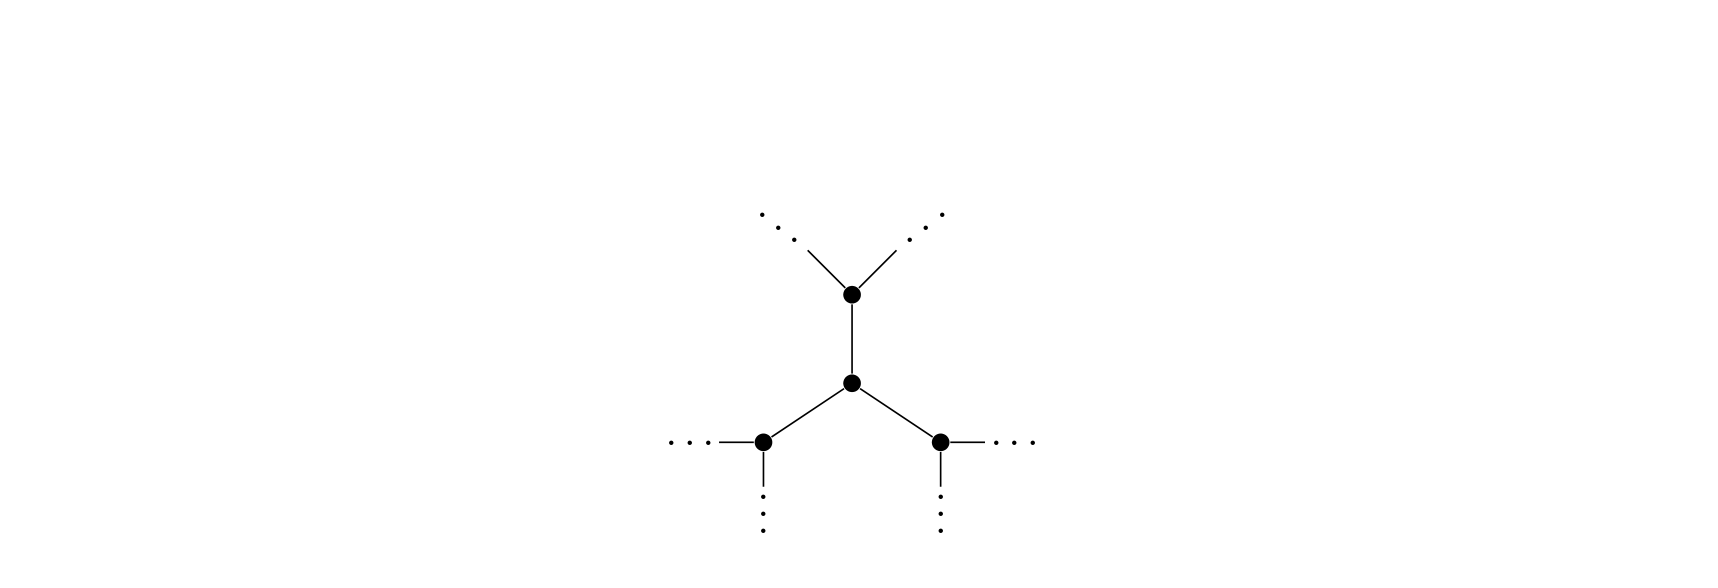
\includegraphics[width=0.4\textwidth]{figure9-1.png}
  \caption{$\mathrm{PGL}_2$在$\Q_2$上的建筑是一棵$3$-正则树。图中画出了构成$\mathrm{PGL}_2/\Q_2$建筑的无限$3$-正则树的$4$个顶点。完整的建筑见图 9.2。（原文 p.~131，Figure 9.1）}
  \label{fig:9-1}
\end{figure}

\begin{figure}[htbp]
  \centering
  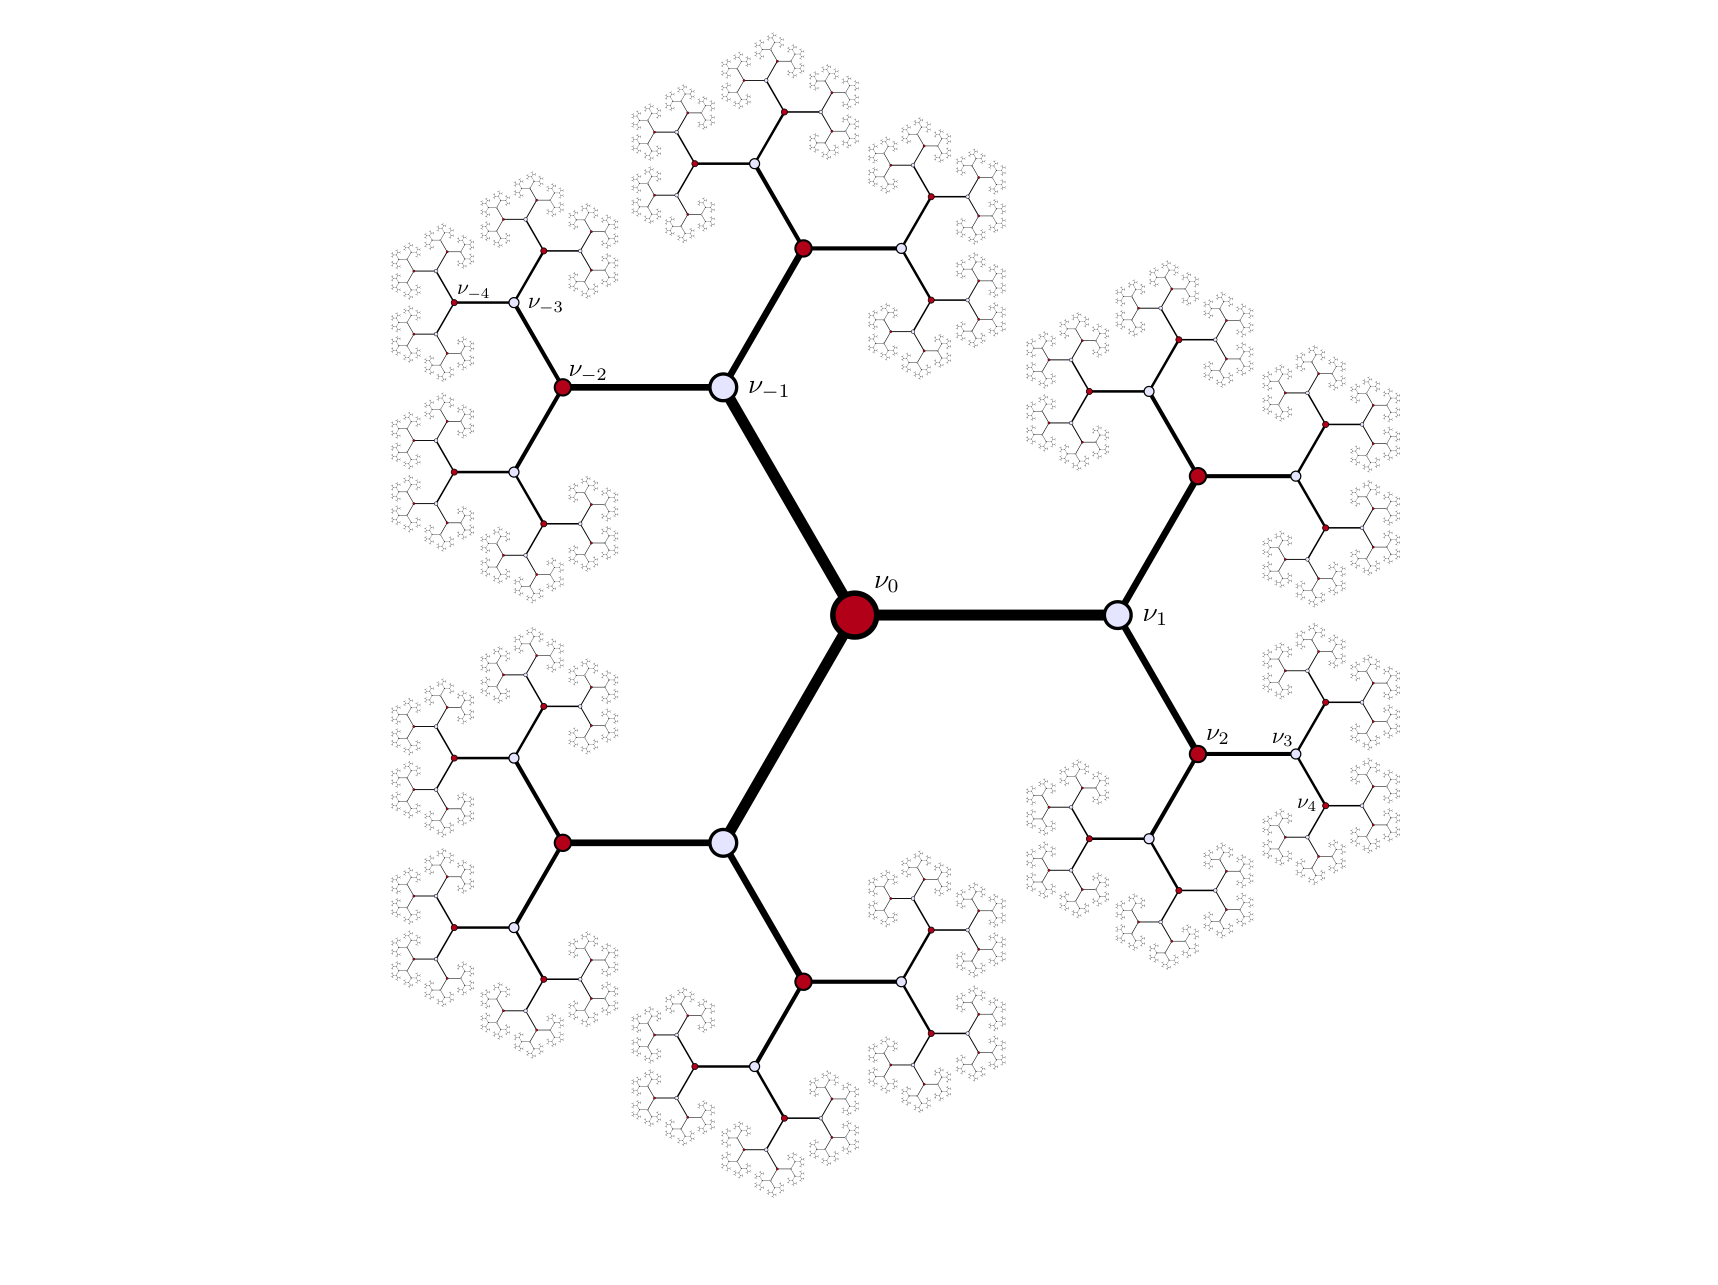
\includegraphics[width=0.78\textwidth]{figure9-2.png}
  \caption{$\mathrm{PGL}_2$在$\Q_2$上的建筑。$G(\cO)$-轨道是围绕中心的同心“圆环”状顶点集，并以颜色区分。图取自 [Cas14]。（原文 p.~131，Figure 9.2）}
  \label{fig:9-2}
\end{figure}

% ---------------------------------------------------------------- 原文 p.132
这也称为$G$的仿射 Grassmann 流形。这是双曲空间的$p$-进类比。想法是顶点在无穷远处聚集，正如双曲空间的圆盘模型。美妙之处在于，双曲空间的许多标准特征都反映在这棵树的几何中。

双商
\begin{equation}\tag{9.127}
G(\cO)\backslash G(K)/G(\cO)
\end{equation}
对应于这棵建筑上的$G(\cO)=\mathrm{PGL}_2(\Z_p)$-轨道。回忆在实际的双曲空间$\mathbb H$中，$i$的稳定化子是$G(\cO)$，其他$G(\cO)$-轨道由它们到某点$i$的距离标记。这里我们有类似的图景。$G(\cO)$是$\Q_p^{2}$中模去伸缩的$\Lambda_0=\Z_p^{2}$的稳定化子，即图 9.1 中间这个点的稳定化子等于$G(\cO)$。然后其他轨道同样是这些同心“圆环”，由到$\Lambda_0$的距离标记，只是现在距离由树度量给出，即边数。所以轨道对应于$\Z_{+}$。

于是 Hecke 算子如下。“树 Laplacian”$T_{p^n}$把$G(K)/G(\cO)$上的函数$f$送到在固定距离$n$的点上取平均的函数：
\begin{equation}\tag{9.128}
(T_{p^n}f)(v)=\sum_{\operatorname{dist}(w,v)=n}f(w).
\end{equation}
同样地，这些全部交换，而且我们发现这些算子的代数就是多项式代数$\C[T_p]$。

所以只要把$\Bun_G$写成
\begin{equation}\tag{9.129}
\Bun_G=G(F)\backslash\prod{}^{\prime}G(K_x)/G(\cO_x),
\end{equation}
我们就得到所有这些代数的作用，且它们彼此交换。目前还不清楚的是：这些代数每一个自身是交换的。
% [Tutor Note: 末句是本章的悬念，也是后续各章的主题：局部 Hecke 代数$\C_c[G(\cO)\backslash G(K)/G(\cO)]$的交换性由 Satake 同构（定理 8）保证，但“整体”Hecke 代数的交换性需要 TFT/几何 Langlands 的解释。阅读时勿把两个层级的交换性混为一谈。]
